\section{System installation guide}
\label{sec:deployment}

The requirements of the project on its hosting platform is shown in Table \ref{tab:req}. Make sure the requirements are met before proceeding to deploy the project.

\setlength{\tabcolsep}{12pt}
\renewcommand{\arraystretch}{1.2}
\begin{table}[h!]
    \centering
    \begin{tabular}{c|c|c}
        Level & OS & Software \\
        \hline\hline
        Minimum& Windows 10; MacOS 10.9; Linux 4.0(kernel) & Python 3.8 \\
        Recommended & Windows 11; MacOS 13; Linux 5.17(kernel) & Python 3.9, 3.10\\
    \end{tabular}
    \caption{Requirements}
    \label{tab:req}
\end{table}
\renewcommand{\arraystretch}{1}
\setlength{\tabcolsep}{0pt}

\begin{enumerate}
\item Make sure having python libarary \mintinline{md}{virtualenv} installed, or install with \mintinline{sh}{pip install virtualenv}.
\item Initialize a new virtualenv and install all dependencies.
\begin{minted}{sh}
python -m venv env                      # create virtual environment
source env/bin/activate                 # activate virtual environment. 
# On Windows, run env\Scripts\activate instead.
pip install -r requirements.txt         # install all dependencies
\end{minted}
\item Initialize the Django database schema.
\begin{minted}{sh}
python manage.py makemigrations marketplace
python manage.py migrate
\end{minted}
\item Creating an admin user \\
First we’ll need to create a user who can login to the admin site. Run the following command:
\begin{minted}{sh}
python manage.py createsuperuser
# Enter your desired username and press enter.
Username: admin
# You will then be prompted for your desired email address:
Email address: admin@example.com
# The final step is to enter your password. 
# You will be asked to enter your password twice, 
# the second time as a confirmation of the first.
Password: **********
Password (again): *********
Superuser created successfully.
\end{minted}
After step 8, open a Web browser and go to “/admin/” on your local domain – e.g., https://127.0.0.1:8000/admin/. You should see the admin’s login screen.
\item Save environmental variables into a \mintinline{md}{.env} file:
\begin{minted}{ini}
# Cloudinary api configurations (available after registration),
# see https://cloudinary.com/
C_NAME = ""
C_KEY = ""
C_SECRET = ""

# email backend configurations
# send to console: "django.core.mail.backends.console.EmailBackend"
# send to mailbox: "django.core.mail.backends.smtp.EmailBackend"
EMAIL_BACKEND = "django.core.mail.backends.console.EmailBackend"

# A mail account as host for sending emails
EMAIL_HOST = ""
EMAIL_HOST_USER = ""
EMAIL_HOST_PASSWORD = ""

# Django Secret key
SECRET_KEY = "<THIS KEY MUST NOT BE EMPTY>"
\end{minted}
\item Make locally-trusted development certificates for https. \\
This tool, \href{https://github.com/FiloSottile/mkcert}{mkcert}, is available to generate the certificate and the key.
\item Run the server on localhost.
\begin{minted}{sh}
python manage.py runserver              # run the server in http
python manage.py runsslserver --certificate cert.pem --key key.pem
                                        # https with local certificate
\end{minted}
\end{enumerate}

By opening the URL shown in the console after running the server (maybe \hyperlink{http://127.0.0.1:8000}{http://127.0.0.1:8000} or \hyperlink{https://127.0.0.1:8000}{https://127.0.0.1:8000}) with browser, a welcome page (e.g., Figure \ref{fig:welcome}) should show up, which indicates completion of deployment.

\begin{figure}[h]
\centering
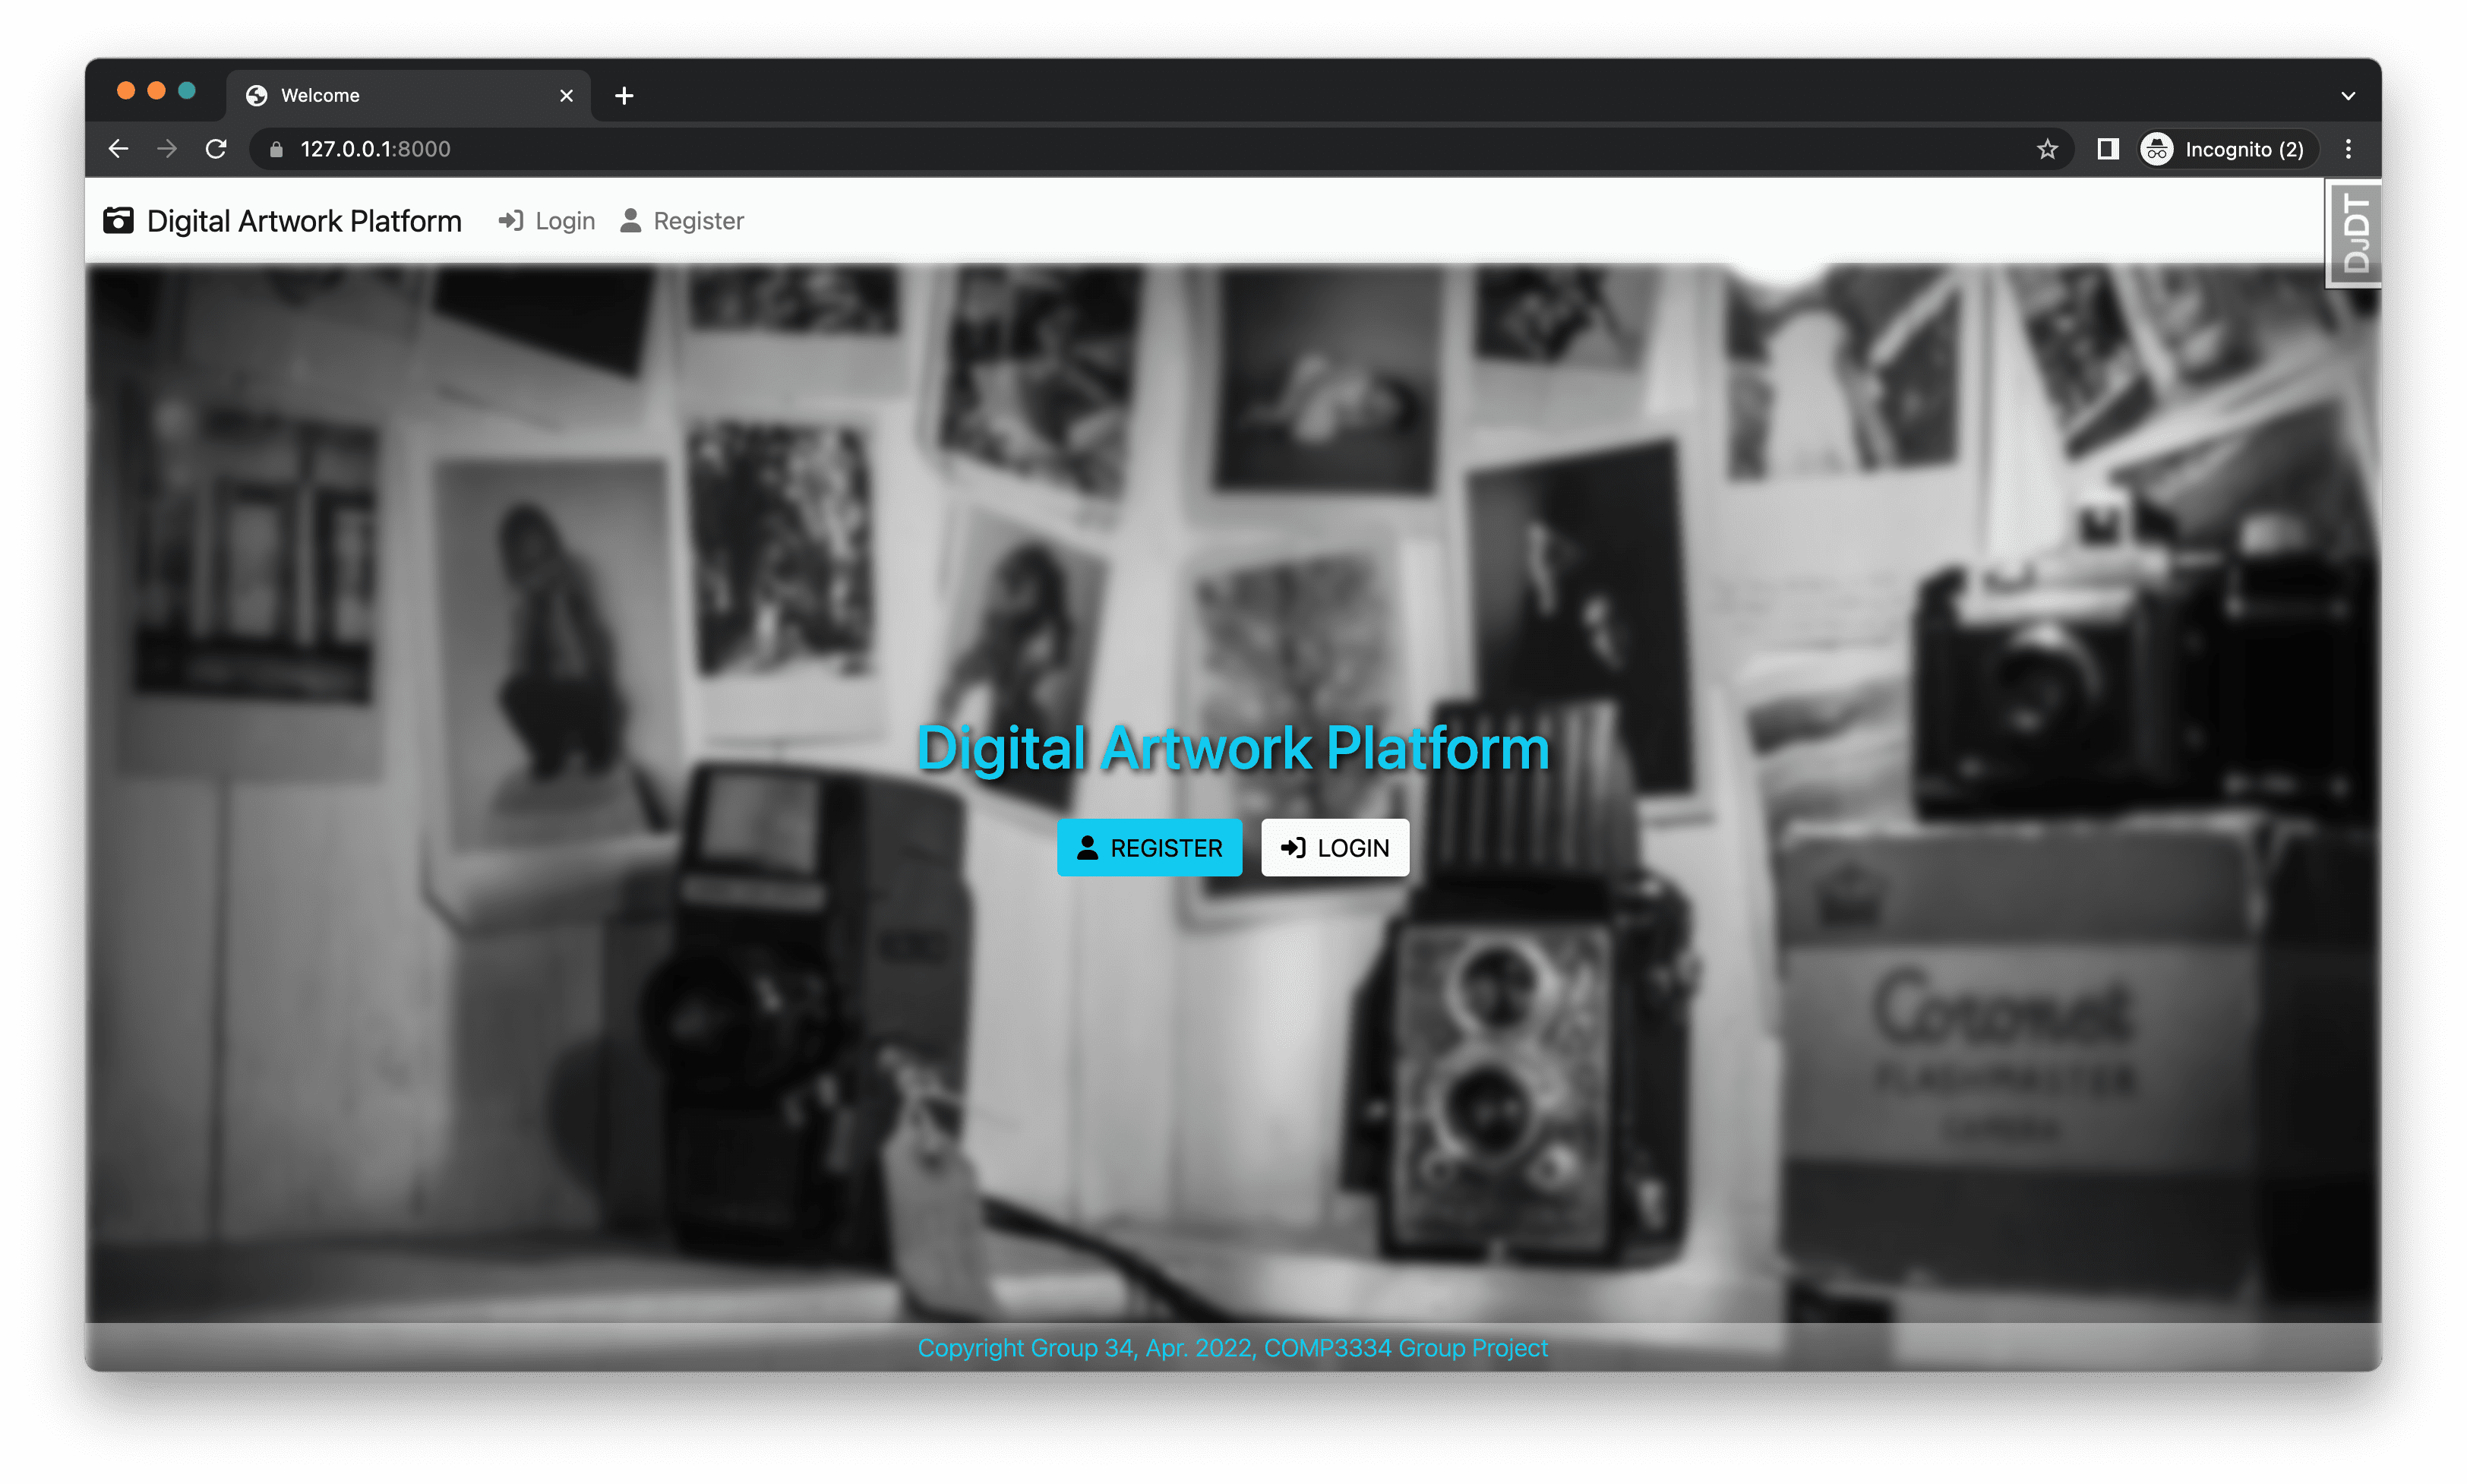
\includegraphics[width=\textwidth]{figures/welcome.png}
\caption{Welcome Page, which indicates success of deployment}
\label{fig:welcome}
\end{figure}
